%%==============================================================================
%% Self-Calibrating Uncertainty-Aware MPC for Tail-Risk Budgeting in Portfolios
%%
%% IEEE JOURNAL manuscript (IEEEtran). Build:
%%     pdflatex paper.tex && bibtex paper && pdflatex paper.tex && pdflatex paper.tex
%%   (or: latexmk -pdf paper.tex)
%%
%% VERIFICATION STATUS -- read before trusting any number here
%% ---------------------------------------------------------------------------
%% Every figure in the tables was recomputed from the committed code on the
%% validation period (2016-01-01..2019-12-31, 983 trading days) on 2026-10-01.
%% NOTHING in the sealed test period (2020-01-01 onward) has been examined.
%% Two numbers an earlier draft asserted were REMOVED because they could not be
%% reproduced from committed code:
%%   1. "5 jump events, 4/5 and 2/5" -- those came from an uncommitted ad-hoc run
%%      (results/fwdvol_jump_events.csv, no script). The committed, hard-bounded
%%      experiments/jump_events.py finds 4 de-clustered events and 3/4 and 1/4.
%%      The paper reports the reproducible 4-event numbers.
%%   2. "pearson corr(fwdvol,|r|) 0.188 vs 0.170" -- NOT robust. Recomputed, the
%%      statistic swings with the fit window (pearson 0.09-0.24, spearman
%%      0.02-0.14 for lookback 400-500), and at the configured lookback=1000 it
%%      cannot be measured on train at all (train is 982 days). The paper
%%      therefore makes no precise correlation claim and rests H3 on the
%%      matched-information decision test instead, which is robust.
%%
%% FIGURE AND TABLE PLACEMENT
%% ---------------------------------------------------------------------------
%%  Fig. 1  teaser / one-page summary   Sec. I    OPTIONAL, commented out below
%%  Fig. 2  system block diagram        Sec. III-A  docs/figures/block_diagram.png   [EXISTS]
%%  Fig. 3  self-calibration loop       Sec. III-D  docs/figures/flow.svg           [EXISTS, stale 2025-09-30 -- regenerate]
%%  Fig. 4  main forest plot            Sec. V-A    *** PLACEHOLDER, must generate ***
%%  Fig. 5  budget utilization          Sec. V-A    *** PLACEHOLDER, must generate ***
%%  Fig. 6  exposure vs CVaR scatter     Sec. V-D    *** PLACEHOLDER, must generate ***
%%  Fig. 7  per-event jump CVaR         Sec. V-E    *** PLACEHOLDER, must generate ***
%%  Tab. I   budget diagnostics         Sec. III-C
%%  Tab. II  full 15-strategy ladder     Sec. V      [VERIFIED]
%%  Tab. III paired bootstrap           Sec. V-A    [VERIFIED]
%%  Tab. IV  forward-vol matched info   Sec. V-C    [VERIFIED]
%%  Tab. V   exposure-matched control   Sec. V-D    [VERIFIED]
%%  Tab. VI  per-event jump study       Sec. V-E    [VERIFIED]
%%  Tab. VII falsified register         Sec. VI     [VERIFIED]  (table*)
%%  Tab. VIII per-year breakdown        App. C      [VERIFIED]
%%  Tab. IX  notation                   App. A
%%==============================================================================
\documentclass[journal]{IEEEtran}

\usepackage[margin=1in]{geometry}
\usepackage{amsmath,amssymb,amsthm,bm}
\usepackage{graphicx}
\usepackage{booktabs}
\usepackage{array}
\usepackage{multirow}
\usepackage{xcolor}
\usepackage{microtype}
\usepackage{url}
\usepackage[hidelinks,breaklinks=true]{hyperref}
\usepackage[nameinlink,noabbrev]{cleveref}

\makeatletter
\renewcommand{\topfraction}{0.92}
\renewcommand{\bottomfraction}{0.7}
\renewcommand{\textfraction}{0.07}
\renewcommand{\floatpagefraction}{0.75}
\makeatother

\newcolumntype{L}[1]{>{\raggedright\arraybackslash}p{#1}}
\newcommand{\ours}[1]{\textcolor{blue!70!black}{\textbf{#1}}}
\newcommand{\best}[1]{\textbf{#1}}

\DeclareMathOperator{\E}{\mathbb{E}}
\DeclareMathOperator{\CVaR}{\mathrm{CVaR}}
\DeclareMathOperator*{\argmin}{arg\,min}
\newcommand{\riskav}{\boldsymbol{\gamma}}
\newcommand{\Rt}{\mathbf{R}}
\newcommand{\w}{\mathbf{w}}
\newcommand{\eps}{\boldsymbol{\epsilon}}
\newcommand{\ind}{\mathbb{I}}

\begin{document}

\title{Self-Calibrating Uncertainty-Aware Model Predictive Control\\
for Tail-Risk Budgeting in Portfolios}

\author{Tenisha~S.%
\thanks{Manuscript draft. All reported results are validation-period
measurements; the test period is sealed and unexamined. Code, configuration, and
the full chronological experiment log accompany this manuscript.}}
\maketitle

\begin{abstract}
Risk limits in portfolio allocation are conventionally a single scalar---a
maximum exposure or a volatility target---which is indifferent to the
\emph{shape} of the loss distribution and cannot react to a forecast that proves
unreliable. We study the alternative: a hard \emph{budget} on the tail, imposed as
an explicit constraint rather than a scaled heuristic. Our contribution is a
controlled instrument comparison, not a performance claim. Holding an entire
learning-and-control stack fixed---online adaptive conformal return intervals, a
breach-feedback coefficient, a convex model-predictive-control allocator---we
swap \emph{only} the risk instrument and add a daily $\CVaR_{5\%}$ budget via the
Rockafellar--Uryasev epigraph over a fixed scenario set. The budget improves
$5\%$ CVaR by $0.00159$ (95\% CI $[0.00101,\,0.00214]$, $p=0.001$), replicated
under a forecast-ablation control ($0.00185$, $p=0.001$), and the constraint is
verifiably live rather than slack. We then report four hypotheses of our own that
the data \emph{falsify}. The learned return forecaster is a pure drag: removing it
leaves risk unchanged ($p=0.606$) at one quarter of the turnover. A
forward-looking jump-augmented GARCH(1,1)-t volatility, given to the
\emph{baseline} as well so the comparison is at matched information, significantly
\emph{improves} the simple rule (CVaR $p=0.001$, max drawdown $p=0.028$) and
significantly makes the MPC \emph{worse} (CVaR $p=0.001$): the MPC dilutes a good
signal. The MPC's residual advantage is not a de-risking artifact---at matched
realized exposure it holds up to $1.18\times$ \emph{more} risk for less return.
The negative results are the substance: in this data the strongest risk
controller we found is the simplest one.
\end{abstract}

\begin{IEEEkeywords}
portfolio optimization, model predictive control, conformal prediction,
conditional value-at-risk, risk budgeting, transaction costs, negative results
\end{IEEEkeywords}

\section{Introduction}
\label{sec:intro}

Risk limits in an institutional allocator are almost always one number: a maximum
exposure, a volatility target, a drawdown-triggered de-scaling. Each collapses
risk into a single scalar and is then tuned. In our experiments this proves very
hard to beat, and understanding why is the point of the paper.

The idea we study is that the \emph{tail} deserves its own instrument. A
portfolio's $5\%$ CVaR is not a function of its volatility: a book of many small
losses and a book containing one large loss can share a volatility and differ
enormously in the tail. A scalar exposure cap cannot distinguish them. A
\emph{tail-risk budget} can, because it constrains the quantity of direct interest
and is falsifiable in a way that a tuned scalar is not.

The second ingredient is that a risk limit ought to respond to \emph{how much we
trust the forecast}. If a predictive interval is wide, the forecast is uncertain,
and a controller that ignores this sizes the same position regardless. We close
the loop: an online adaptive-conformal layer produces per-asset intervals, a
learned coefficient updates from observed interval breaches, and both feed the
risk instrument.

This yields a question we believe is under-asked: when one has a learned forecast
\emph{and} an optimizer, does the \emph{shape} of the risk limit matter? The
forecast machinery, the optimizer, the cost model, and the data are all held
fixed; only the risk instrument changes. Our answer: the instrument matters, and
the tail is the right one---but relative to the machinery it is added to, not
relative to a competent volatility-targeting baseline. That distinction is the
paper, and \cref{sec:falsified} states it without hedging.

\subsection{Contributions}
\label{sec:contrib}

\begin{enumerate}
\item \textbf{A tail-risk budget as a first-class MPC constraint.} A daily
$\CVaR_{5\%}$ budget via the Rockafellar--Uryasev epigraph over a fixed scenario
set, calibrated on training data so the constraint is \emph{live} at full
investment rather than slack (\cref{sec:budget}). Added to the identical
uncertainty-driven exposure cap, the budget improves $5\%$ CVaR at $p=0.001$,
replicated under forecast-ablation control.
\item \textbf{A self-calibrating uncertainty loop that is verifiably active.} Online
adaptive conformal intervals per asset, a learned breach-feedback coefficient, and
a geometric uncertainty ratio driving the budget. We report achieved coverage and
the distribution of constraint utilization, and show the loop is not inert.
\item \textbf{Negative results, documented rather than buried.} Four
self-generated hypotheses are falsified (\cref{sec:falsified}), each with a paired
stationary-bootstrap significance statement, two of them significant at $p=0.001$
in \emph{opposite} directions at matched information.
\item \textbf{A reproducibility discipline that made (3) possible.} Every strategy
shares data, period, costs, and lookback; a no-look-ahead test runs for every new
feature; a regime-search bound is unit-tested so a sealed-period event cannot be
selected by accident; and four parameterization traps in the volatility model are
recorded (\cref{app:traps}), because each produced a plausible-looking yet
worthless signal.
\end{enumerate}

% ---- OPTIONAL Fig. 1: teaser, top of first column in Sec. I --------------
% \begin{figure}[!t]
%   \centering
%   \includegraphics[width=\columnwidth]{docs/figures/teaser.pdf}
%   \caption{One-page summary: the mechanism, the controlled instrument
%   comparison, and the four falsified hypotheses.}
%   \label{fig:teaser}
% \end{figure}

\section{Related Work}
\label{sec:related}

\subsection{Conformal prediction under distribution shift}
Angelopoulos and Bates~\cite{angelopoulos2023gentle} give a tutorial treatment of
the conformal framework, and Gibbs and Cand\`es~\cite{gibbs2021adaptive} establish
the adaptive-conformal-inference update we use for online interval calibration.
We adopt the standard ACI update directly and claim no new conformal result; our
contribution is to route the resulting interval width into a \emph{risk
constraint} rather than a scaling heuristic.

\subsection{Conformal uncertainty meets model-based control}
This is the nearest prior work and a reviewer will rightly ask about it. Chee et
al.~\cite{chee2024uncertainty} use conformal regions to tighten constraints in
model-based controllers, and Richards and How~\cite{richards2006robust} establish
the constraint-tightening convention our \texttt{tighten\_limits} follows. Chee et
al.\ work in continuous control rather than portfolio allocation, and their
tightening is driven by a disturbance bound rather than by a calibrated online
interval. The difference here is the source of the tightening signal: an adaptive
conformal return interval updated online, per asset. We regard Chee et al.\ as the
closest methodological neighbour and do not claim novelty for conformal-driven
tightening per se; our claim is about the \emph{instrument} being tightened to.

\subsection{Risk budgeting, CVaR, and coherent risk measures}
Rockafellar and Uryasev~\cite{rockafellar2000optimization} established the
formulation used in \cref{eq:budget}. Artzner et al.~\cite{artzner1999coherent}
ground the economic case for coherent tail measures, and Markowitz
\cite{markowitz1952portfolio} remains the mean--variance point of departure.
DeMiguel et al.~\cite{demiguel2009optimal} show how hard it is to beat $1/N$
diversification, which is why we add equal-weight and volatility-targeting
baselines before building any adaptive layer.

\subsection{Convex MPC allocation}
Rawlings et al.~\cite{boyd2004convex} and Combettes and Pesquet
\cite{combettes2011proximal} supply the convex-programming and
duality/proximal machinery behind the allocator. The program here is a
short-horizon risk-constrained convex quadratic program, so the MPC is an
allocation with a risk constraint rather than a long-horizon trajectory
optimization. Ledoit and Wolf~\cite{ledoit2004well} motivate the shrunk covariance
estimate feeding the objective.

\subsection{Decision-focused learning}
The closest methodological neighbour is decision-focused learning, which optimizes
a differentiable surrogate of the \emph{decision} loss rather than a forecast
error: Donti et al.~\cite{donti2017task} introduce the end-to-end task-based
formulation, and Sadana et al.~\cite{sadana2023contextual} survey contextual
optimization under decision uncertainty. A pilot of this family was explicitly
out of scope for our project and is \emph{not} implemented here. We nonetheless
consider it the nearest conceptual neighbour, because it reports the same
phenomenon we do from the opposite direction: decision-aware machinery can be
neutral or actively harmful relative to a well-specified simple rule.

\subsection{Volatility-managed portfolios and regime switching}
Moreira and Muir~\cite{moreira2017volatility} show that volatility scaling
substantially improves Sharpe ratios for well-known factors; Barroso and
Santa-Clara~\cite{barroso2015momentum} reach a compatible conclusion for equity
momentum. This is the direct motivation for our strongest baseline and, in
\cref{sec:forward}, for the finding that it is the strongest risk controller we
found. Hamilton~\cite{hamilton1989new} is the regime-switching precedent for the
calm/stress layer in our system; our implementation is a far simpler
rolling-volatility detector rather than a Markov model, which we describe as a
deviation. Politis and Romano~\cite{politis1994stationary} supply the stationary
block bootstrap used for all inference, since the i.i.d.\ bootstrap is invalid for
dependent return series.

\subsection{Position of this work}
Our result is deliberately narrower than a performance claim. We do not show that
MPC beats volatility targeting; we show that \emph{given} this allocator, adding a
tail budget improves the tail relative to the identical allocator without one, and
we document the conditions under which the added MPC structure does not help. The
nearest work on decision-focused learning reaches a compatible conclusion---extra
decision-aware machinery is not automatically beneficial---and we differ in
setting and in the specific object isolated: the risk \emph{instrument}.

\section{Method}
\label{sec:method}

\subsection{System overview}
\Cref{fig:blocks} shows the system. The daily loop: historical returns $\Rt_d$
available at the close of day $d$; a return forecaster producing $\hat{\mu}_d$ and
adaptive conformal intervals with half-widths $\mathbf{h}_d$; a self-calibration
module mapping observed breaches to a scalar $\beta_d$; a risk-budget stage mapping
uncertainty to a daily CVaR budget; and a convex MPC producing target weights
$\w_d$, which the engine executes at cost $b\lVert\Delta\w\rVert_1$ with $b=10$
basis points per unit turnover, in \emph{every} backtest including baselines.

\begin{figure}[!t]
  \centering
  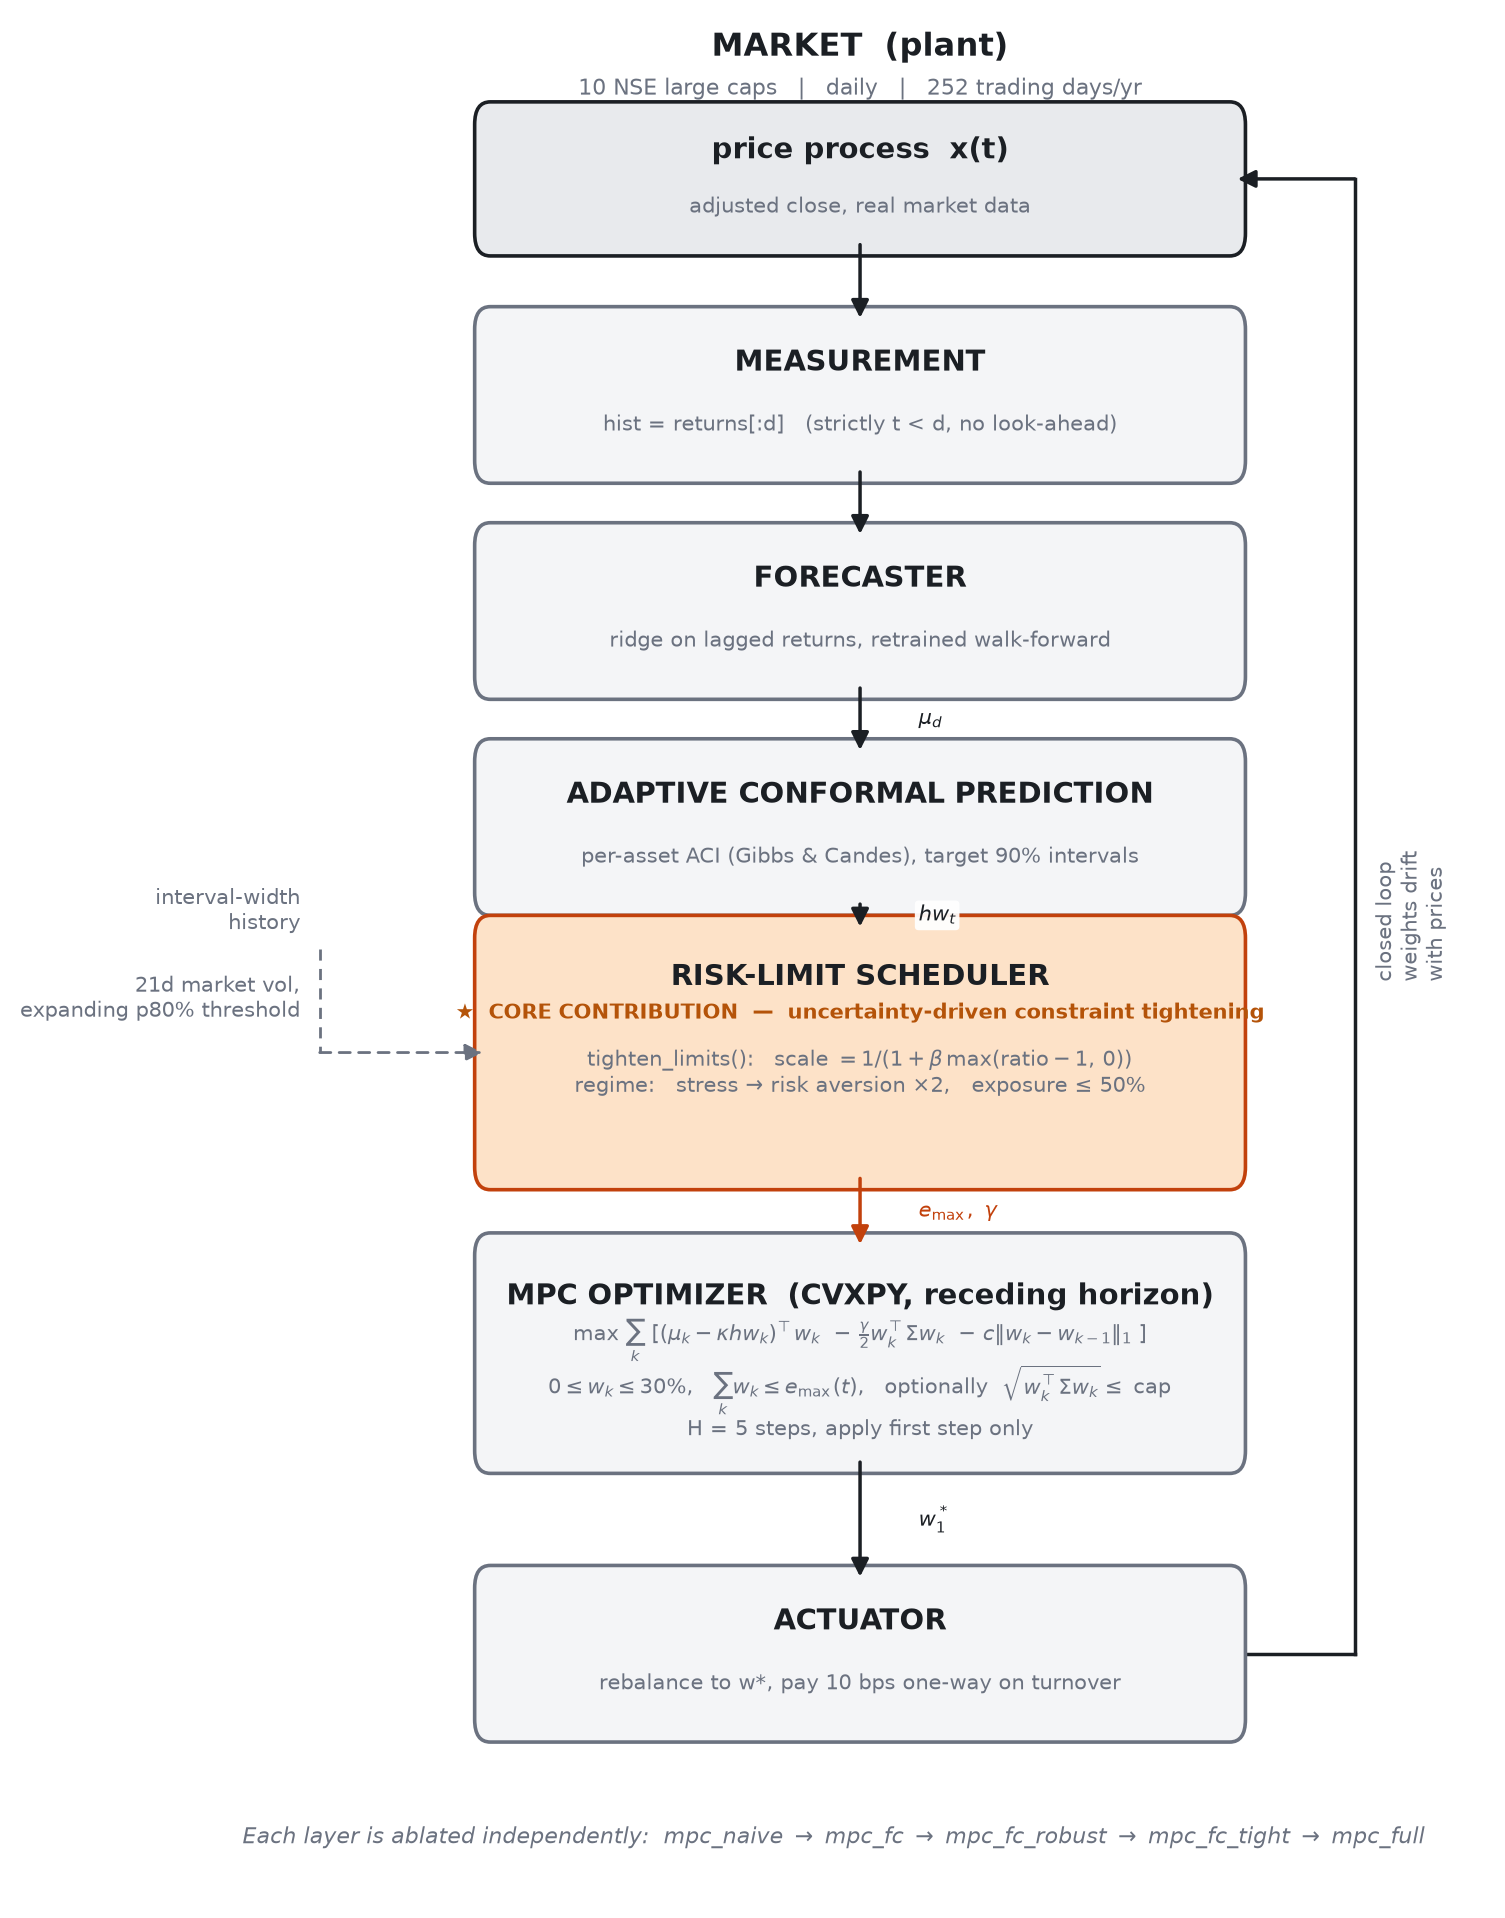
\includegraphics[width=\columnwidth]{docs/figures/block_diagram.png}
  \caption{System block diagram, rendered directly from the live configuration so
  it cannot drift from the implemented pipeline.}
  \label{fig:blocks}
\end{figure}

\subsection{Convex MPC allocation with conformal forecasts}
\label{sec:mpc}

At day $d$ the allocator solves
\begin{equation}
\label{eq:mpc}
\w_d^\star = \argmin_{\w}\ \frac{\riskav}{2}\,\w^\top\Vt_d\w
- \mathbf{m}_d^\top\w,
\end{equation}
subject to $\w\in\mathbb{R}^N_+$, $\mathbf{1}^\top\w \le e_{\max}$,
$\lVert\w\rVert_2 \le v_{\max}$. Here $\Vt_d$ is a shrunk covariance estimate
(\cite{ledoit2004well}), $\mathbf{m}_d$ is the mean forecast shrunk toward zero,
and $e_{\max},v_{\max}$ are the uncertainty-driven limits of the exposure-cap
instrument. Because the scenario shocks are fixed, the tail objective in
\cref{eq:budget} is \emph{linear} in $\w$, so the program stays a quadratic
program.

\subsection{The tail-risk budget}
\label{sec:budget}

Let the daily loss under fixed scenario $r$ be
$\ell_r(\w)=-\w^\top\eps_r$. The empirical CVaR of $\ell$ over $R$ equiprobable
scenarios at level $\alpha$ admits the Rockafellar--Uryasev representation
\begin{equation}
\label{eq:ru}
\min_{\mathbf{u}\ge 0}\ \mathbf{1}^\top\mathbf{u}
\quad\text{s.t.}\quad
u_r \ge \ell_r(\w),\ \ r=1,\dots,R,
\end{equation}
which equals $\CVaR_\alpha(\ell(\w))$ at the optimum. We impose the hard daily
budget
\begin{equation}
\label{eq:budget}
\mathbf{1}^\top\mathbf{u} \;\le\; \alpha\,\text{budget}_t,
\qquad
\text{budget}_t = m_v\,\sigma_t\,\text{scale}_t,
\qquad
\text{scale}_t = \frac{1}{1+\beta_t\max(\text{ratio}_t-1,\,0)},
\end{equation}
with $\text{scale}_t$ floored at $s_{\min}$. Here $m_v$ is a volatility
multiplier, $\sigma_t$ the equal-weight volatility over the lookback, $\beta_t$ the
learned breach-feedback coefficient, and $\text{ratio}_t$ the conformal-width /
ensemble-disagreement uncertainty ratio. Two implementation details are
load-bearing. First, the $1/\alpha$ factor in \cref{eq:budget} must match the
epigraph scaling in \cref{eq:ru}: dropping it inflates the CVaR term and yields
over-budget solutions. Second, an infeasible budget must fall back to
\textbf{cash}, never to the previous weights, which are fully invested---the
opposite of risk-off.

We set $\alpha=0.05$, $R=200$, and calibrate $m_v$ on \textbf{training data only}
from the observed ratio of realized CVaR to volatility, choosing $m_v=1.6$ so the
budget sits just under the observed tail. \Cref{tab:budgetdiag} confirms the
constraint is live.

\begin{table}[!t]
  \centering
  \caption{Budget diagnostics, validation period ($983$ days). Utilization is the
  share of the budget consumed, $\CVaR_{\text{used}}/\text{budget}$. A budget that
  never binds is not a result, so we report the whole distribution; "binding" is
  utilization $\ge 0.98$. Mean budget is $0.01387$ for both strategies.}
  \label{tab:budgetdiag}
  \begin{tabular}{lcccc}
    \toprule
    Strategy & Mean util. & Median util. & Max util. & Binding days \\
    \midrule
    \texttt{mpc\_tailbudget}        & 0.869 & 0.985 & 0.995 & 54.2\% \\
    \texttt{mpc\_tailbudget\_nofc}  & 0.837 & 0.984 & 0.997 & 52.5\% \\
    \bottomrule
  \end{tabular}
\end{table}

The budget binds on $54.2\%$ of validation days, with \textbf{zero violations} in
$983$ days and maximum utilization $0.995$. We solve with a real interior-point
method at tight tolerances: at default settings the solver returned an
\texttt{optimal\_inaccurate} status while violating the budget by roughly $20\%$,
which is precisely the silent failure that motivates a violation counter in the
result logs.

\subsection{What ``self-calibrating'' does and does not mean}
\label{sec:selfcal}

The feedback loop is verifiably \emph{active}: realized interval-breach frequency
is $0.0112$ against a target $\delta=0.01$. Its effect on realized exposure is
nevertheless small, and we say so plainly rather than presenting the loop as
though it delivered large gains. The geometric ratio requires \emph{both} the
conformal arm and the ensemble-disagreement arm to move before the budget shrinks,
and $\delta=0.01$ starves the loop of feedback, yielding only $11$ breaches in $983$
days. The measured mean exposure cap is $0.991$ and the mean uncertainty ratio
$1.016$: there is almost nothing to tighten. This is a design limitation with an
obvious fix (larger $\delta$, or an arithmetic rather than geometric combination);
we did not adopt it, because tuning the loop against validation returns would
invalidate the held-out discipline the rest of this paper depends on.

% ---- Fig. 3: loop detail, top of a column in Sec. III-D ------------------
\begin{figure}[!t]
  \centering
  % NOTE: flow.svg is stale (2025-09-30) and predates the forward-vol and
  % exposure-control workstreams. Regenerate from docs/flow.mmd before submission.
  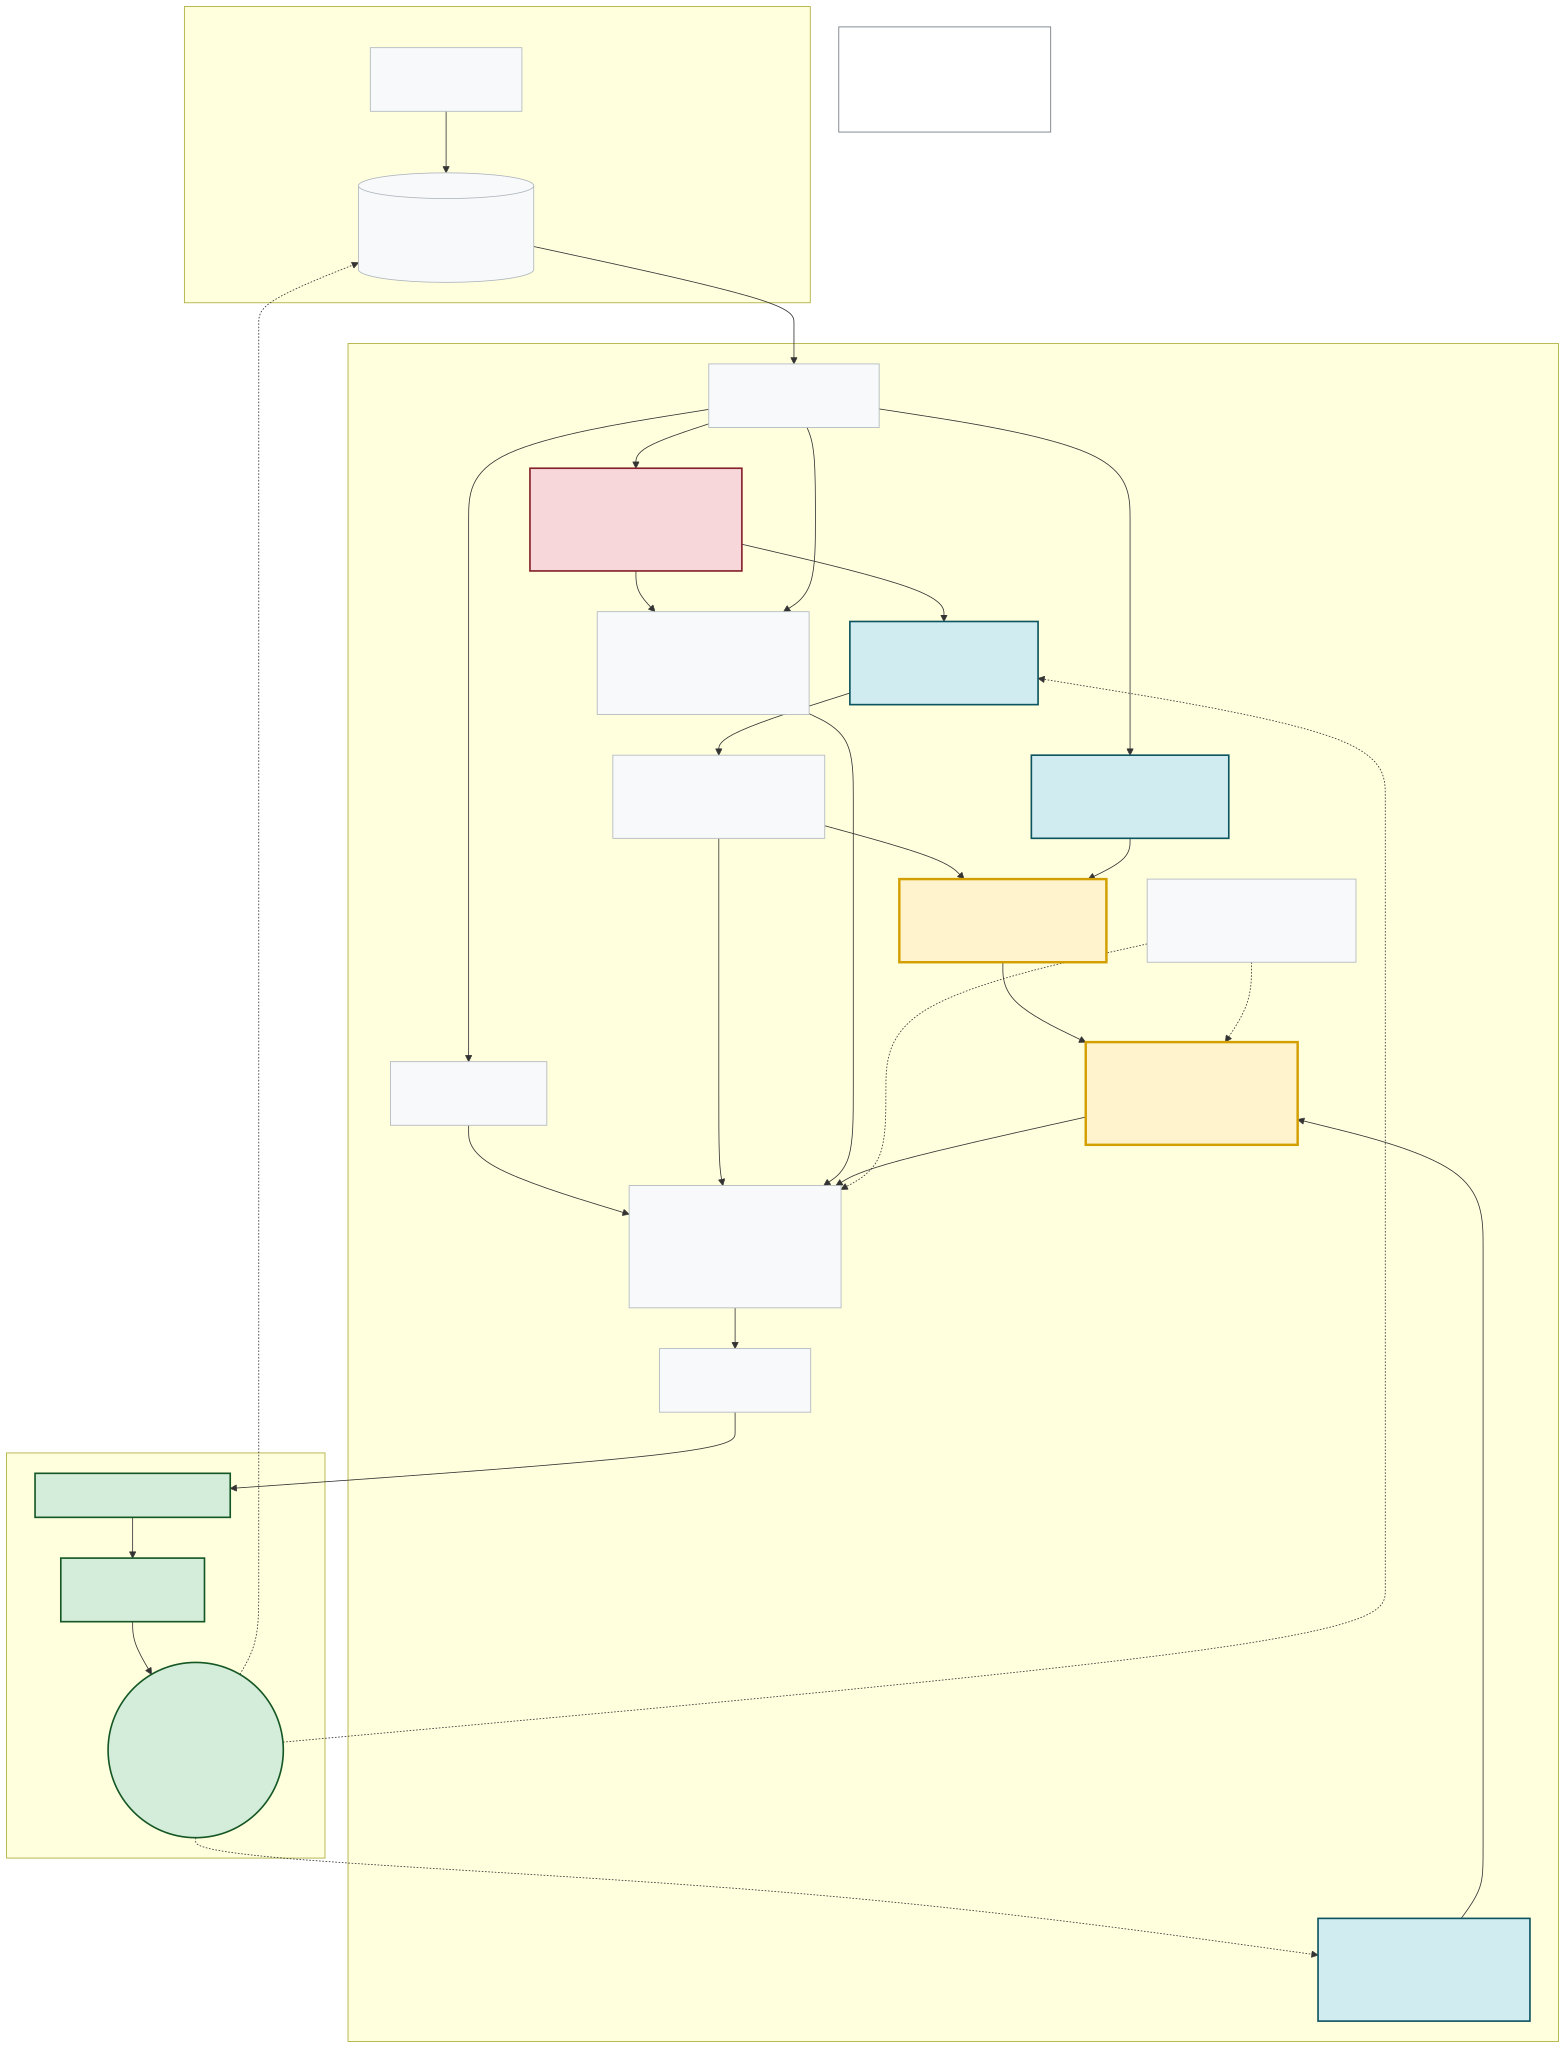
\includegraphics[width=\columnwidth]{docs/figures/flow.svg}
  \caption{Detail of the self-calibrating uncertainty loop. Conformal half-widths
  and ensemble disagreement enter a geometric ratio; the learned coefficient
  $\beta_t$ updates from realized interval breaches and scales the CVaR budget.}
  \label{fig:loop}
\end{figure}

\subsection{Forward-looking volatility for the matched-information test}
\label{sec:fwdmethod}

To test whether the budget loses because it is denominated in \emph{trailing}
volatility, we fit a jump-augmented GARCH(1,1) with Student-$t$ innovations by
maximum likelihood on a trailing window, re-estimating every $20$ days. The
conditional variance
$h_{t+1}=\omega+\alpha\epsilon_t^2+\beta h_t$, with an extra multiplicative shock
on jump days flagged by a $|\epsilon|$ quantile, reacts to the newest shock, which
a $60$-day trailing window cannot do at full speed. It is delivered to \emph{both}
the MPC and the scalar baseline so that \cref{sec:forward} is a test at matched
information. Four implementation traps, each of which produced a worthless signal
while looking entirely plausible, are documented in \cref{app:traps}.

\section{Experimental Design}
\label{sec:design}

\paragraph{Data and splits.} Ten NSE large caps, daily close. Training
$2012$-$2015$, validation $2016$-$01$-$01$ to $2019$-$12$-$31$ ($983$ trading
days). Everything from $2020$ onward is \textbf{sealed and unexamined}. A
simulated generator exists solely so the test suite runs offline; every parameter
is in the released configuration and the runner prints a warning banner on
simulated runs. No reported number uses it.

\paragraph{Costs, lookback, seed.} Transaction costs of $10$ basis points per unit
turnover apply in every backtest, baselines included. All strategies share the
same lookback, cost model, and random seed ($42$). Every run saves its
configuration alongside its results.

\paragraph{The strategy ladder.} Fifteen strategies, reported in full in
\cref{tab:ladder}. The ablation ladder is ordered so each step adds exactly one
mechanism: \texttt{mpc\_fc} adds the forecaster, \texttt{mpc\_fc\_robust} adds
conformal intervals, \texttt{mpc\_fc\_tight} adds uncertainty-driven tightening,
\texttt{mpc\_selfcal} adds learned breach feedback, and
\texttt{mpc\_tailbudget} adds the tail budget. \texttt{mpc\_tailbudget} is
implemented as a subclass of \texttt{mpc\_selfcal}, so the two differ \emph{only}
by the budget constraint: this is what makes \cref{tab:bootstrap} a clean
instrument comparison.

\paragraph{Two controls that make the negative results credible.}
\texttt{mpc\_tailbudget\_nofc} removes the return forecast and changes nothing
else, so forecast-on versus forecast-off is attributable to the forecast alone.
\texttt{equal\_weight\_voltarget\_fwd} is a \emph{matched-information} control: a
scalar volatility-targeting rule driven by the \emph{same} forward volatility as
the MPC. Without it, a ``win'' for the MPC would show only that a good signal
beats no signal.

\paragraph{Inference.} Paired stationary block bootstrap
\cite{politis1994stationary}, $2000$ resamples, mean block $10$ days, seed $42$,
on the difference in daily net returns. We report the point estimate, a $95\%$
percentile interval, and a two-sided bootstrap $p$-value, and we do not treat an
unadjusted $p$-value from one comparison as a discovery: every headline claim is
either replicated under a second control or stated as a null.

\begin{table*}[!t]
  \centering
  \caption{Complete strategy ladder, validation period ($2016$-$01$-$01$ to
  $2019$-$12$-$31$, $983$ days, costs included). \ours{MPC}$_{\text{budget}}$ is
  the proposed instrument; \texttt{voltarget\_fwd} is the strongest baseline.
  Best per column in bold. Exposure is realized mean gross exposure, reported
  because it confounds the tail metric (\cref{sec:exposure}). $c_\alpha$ is the
  daily $5\%$ CVaR, a negative loss magnitude, so \emph{less negative is better}.}
  \label{tab:ladder}
  \begin{tabular}{lrrrrrrrrr}
    \toprule
    Strategy & Sharpe & Sortino & Ann.\ ret. & Ann.\ vol & $c_\alpha$ &
    MaxDD & Turnover & Cost & Exposure \\
    \midrule
    \texttt{equal\_weight}              & 1.385 & 2.190 & 0.200 & 0.138 & $-0.0172$ & $-0.131$ & 0.011 & 1.08\% & 1.000 \\
    \texttt{buy\_hold}                  & 1.325 & 2.076 & 0.186 & 0.136 & $-0.0170$ & $-0.131$ & 0.001 & 0.10\% & 1.000 \\
    \texttt{markowitz}                  & 0.967 & 1.458 & 0.141 & 0.148 & $-0.0199$ & $-0.156$ & 0.093 & 9.14\% & 0.959 \\
    \texttt{equal\_weight\_voltarget}   & 1.302 & 2.062 & 0.140 & 0.105 & $-0.0131$ & $-0.107$ & 0.014 & 1.34\% & 0.767 \\
    \texttt{mpc\_naive}                 & 1.252 & 1.856 & 0.157 & 0.123 & $-0.0170$ & $-0.155$ & 0.008 & 0.78\% & 0.848 \\
    \texttt{mpc\_dd\_riskaversion}      & 1.103 & 1.610 & 0.125 & 0.113 & $-0.0158$ & $-0.152$ & 0.010 & 0.97\% & 0.767 \\
    \texttt{mpc\_fc}                    & 1.124 & 1.670 & 0.142 & 0.125 & $-0.0171$ & $-0.156$ & 0.035 & 3.43\% & 0.876 \\
    \texttt{mpc\_fc\_robust}            & 1.115 & 1.651 & 0.138 & 0.122 & $-0.0170$ & $-0.155$ & 0.033 & 3.25\% & 0.847 \\
    \texttt{mpc\_fc\_tight}             & 1.073 & 1.587 & 0.127 & 0.118 & $-0.0163$ & $-0.147$ & 0.033 & 3.26\% & 0.815 \\
    \texttt{mpc\_selfcal}               & 1.091 & 1.615 & 0.132 & 0.120 & $-0.0166$ & $-0.152$ & 0.036 & 3.50\% & 0.839 \\
    \midrule
    \ours{\texttt{mpc\_tailbudget}}         & 1.196 & 1.773 & 0.135 & 0.111 & $-0.0150$ & $-0.146$ & 0.036 & 3.54\% & 0.812 \\
    \ours{\texttt{mpc\_tailbudget\_nofc}}   & \best{1.265} & \best{1.898} & 0.143 & 0.111 & $-0.0148$ & $-0.147$ & \best{0.009} & \best{0.89\%} & 0.767 \\
    \ours{\texttt{mpc\_tailbudget\_fwdvol}} & 1.241 & 1.856 & \best{0.146} & 0.116 & $-0.0156$ & $-0.155$ & 0.010 & 1.02\% & 0.784 \\
    \texttt{equal\_weight\_voltarget\_fwd} & 1.299 & 2.033 & 0.123 & \best{0.093} & \best{$-0.0117$} & \best{$-0.094$} & 0.011 & 1.11\% & 0.686 \\
    \texttt{mpc\_full}                  & 1.160 & 1.725 & 0.129 & 0.110 & $-0.0151$ & $-0.136$ & 0.033 & 3.28\% & 0.767 \\
    \bottomrule
  \end{tabular}
\end{table*}

\section{Results}
\label{sec:results}

\subsection{Adding a tail budget to the same allocator improves the tail}

\Cref{tab:bootstrap} isolates the claim in our title. \texttt{mpc\_tailbudget} and
\texttt{mpc\_selfcal} are the same class of allocator with the same
uncertainty-driven exposure cap; they differ only by the CVaR budget. Adding the
budget improves $5\%$ CVaR at $p=0.001$. Both rows are MPC-against-MPC instrument
comparisons, so the forecast, the conformal layer, the tightening rule, the solver,
and the cost model are all held fixed.

\begin{table}[!t]
  \centering
  \caption{Paired stationary block bootstrap on validation ($2000$ resamples,
  mean block $10$ days). $\Delta c_\alpha$ is the CVaR difference in
  less-negative-is-better units, so a \emph{positive} mean favours the
  first-named strategy. The first two rows are the instrument comparison; the
  matched-information rows are the H3 test.}
  \label{tab:bootstrap}
  \begin{tabular}{L{5.6cm}rrc}
    \toprule
    Comparison & $\Delta c_\alpha$ & 95\% CI & $p$ \\
    \midrule
    \ours{budget $-$ self-calibrated cap} & $+0.00159$ & $[0.00101,\,0.00214]$ & \ours{0.001} \\
    \ours{budget $-$ cap (forecast off)}  & $+0.00185$ & $[0.00108,\,0.00268]$ & \ours{0.001} \\
    \midrule
    budget $-$ budget (no forecast)      & $+0.00025$ & $[-0.00050,\,0.00112]$ & 0.606 \\
    budget (no fc) $-$ voltarget         & $-0.00168$ & $[-0.00423,\,0.00056]$ & 0.142 \\
    \midrule
    \ours{fwd-vol scalar $-$ trailing scalar} & $+0.00145$ & $[0.00087,\,0.00195]$ & \ours{0.001} \\
    \ours{MPC (fwd vol) $-$ fwd-vol scalar}  & $-0.00395$ & $[-0.00692,\,-0.00143]$ & \ours{0.001} \\
    budget (no fc) $-$ fwd-vol scalar   & $-0.00313$ & $[-0.00583,\,-0.00086]$ & 0.005 \\
    \bottomrule
  \end{tabular}
\end{table}

% ---- Fig. 4: main forest plot, top of first column in Sec. V-A -----------
% GENERATE: from results/<run>/paired.csv, plot point_diff with 95% CI for the
% CVaR row of each comparison, vertical line at 0. Positive = first-named better.
\begin{figure}[!t]
  \centering
  \framebox[.94\columnwidth]{%
    \parbox[c][5.0cm][c]{.90\columnwidth}{\centering\small
    \textit{PLACEHOLDER --- generate before submission.}\\
    Forest plot of $\Delta c_\alpha$ with 95\% bootstrap intervals for the
    comparisons in \cref{tab:bootstrap}, vertical line at zero, from
    \texttt{results/<run>/paired.csv}.\\
    The point of the figure: only the two instrument rows sit on the positive
    side of zero, and the matched-information rows sit decisively on the
    negative side.}}
  \caption{Main result. The only comparisons that improve on the machinery they
  are added to are the two instrument rows; against a matched-information scalar
  rule every MPC variant is significantly worse.}
  \label{fig:main}
\end{figure}

\subsection{The learned forecaster is a pure drag}
\label{sec:drag}

The return forecaster has no skill on these names: mean per-asset correlation
between prediction and realization is $\approx-0.035$ on $2018$-$2019$, while the
true daily AR(1) coefficient averages $\approx 0.004$. Sharpe degrades
monotonically in the forecast-shrinkage parameter, consistent with the forecast
being near-noise.

The isolating control confirms it. \texttt{mpc\_tailbudget\_nofc} reproduces
\texttt{mpc\_tailbudget} to within noise on every risk metric (CVaR $p=0.606$,
Sharpe $p=0.622$, max drawdown $p=0.869$) while cutting turnover from $0.036$ to
$0.009$ and cost from $3.54\%$ to $0.89\%$. The forecaster buys nothing and costs
roughly four times the trading. We do not claim it adds alpha; the defensible
claim is that the conformal and tightening machinery makes an unreliable
forecaster \emph{safe} to place in the loop, not that it is useful.

\subsection{Forward-looking volatility at matched information}
\label{sec:forward}

If the budget loses because it is denominated in trailing volatility, the remedy is
a forward-looking risk signal. We give the GARCH signal of \cref{sec:fwdmethod} to
\emph{both} the MPC and the scalar baseline. \Cref{tab:forward} shows it improves
the simple rule and degrades the MPC.

\begin{table}[!t]
  \centering
  \caption{Forward-looking volatility at matched information. The MPC and the
  baseline consume the identical GARCH signal, so this isolates what the MPC
  \emph{adds} rather than showing that a good signal beats no signal. All $c_\alpha$
  values are positive loss magnitudes, lower is better.}
  \label{tab:forward}
  \begin{tabular}{lrrr}
    \toprule
    Strategy & $c_\alpha$ & Sharpe & MaxDD \\
    \midrule
    \texttt{voltarget} (trailing vol)     & 0.0131 & 1.302 & $-0.107$ \\
    \texttt{voltarget\_fwd} (GARCH)       & \best{0.0117} & 1.299 & \best{$-0.094$} \\
    \ours{\texttt{mpc\_budget}} (trailing) & $-$0.0150 & 1.196 & $-0.146$ \\
    \ours{\texttt{mpc\_nofc}} (trailing)   & 0.0148 & 1.265 & $-0.147$ \\
    \ours{\texttt{mpc\_fwdvol}} (GARCH)    & 0.0156 & 1.241 & $-0.155$ \\
    \bottomrule
  \end{tabular}
\end{table}

Both directions are significant and they point opposite ways. Against the
trailing-vol scalar rule, the forward signal significantly improves the scalar rule
(CVaR $p=0.001$, max drawdown $p=0.028$). Against that same improved scalar rule,
the MPC consuming the identical signal is significantly worse (CVaR
$-0.00395$, $p=0.001$). On the four de-clustered real jump events of
\cref{sec:jump}, the forward signal helps the scalar rule in $3/4$ and the MPC in
$1/4$. Every MPC variant lands worse than the single scalar rule. The added MPC
structure appears to \emph{dilute} a good signal, converting a good scalar risk
estimate into a worse allocation decision. A useful caveat on the signal itself:
its standalone predictive correlation for $|r_{t+1}|$ is weak and unstable across
fit windows, so we rest this section on the decision-level matched-information
test rather than on any single correlation coefficient.

\subsection{The residual edge is not de-risking}
\label{sec:exposure}

The MPC wins exactly one calendar year of four (2016) and one jump event of four,
and each case looks like the same thing: a falling market. The natural worry is
that the MPC wins the tail metric by holding less risk. We measured realized mean
gross exposure from the backtest weights and rescaled every strategy to a common
exposure. \Cref{tab:exposure} reports both.

\begin{table}[!t]
  \centering
  \caption{Exposure-matched control. Left: realized mean gross exposure. Right:
  all strategies rescaled to a common exposure of $0.686$. The MPC holds
  \emph{more} risk than the baseline and remains worse after matching, so its
  advantage is not a de-risking artifact. Rescaling is an analytical normalization
  (cash at $0\%$), not a tradeable backtest; turnover and cost do not rescale
  consistently, so no cost conclusion is drawn here.}
  \label{tab:exposure}
  \begin{tabular}{lrrrrr}
    \toprule
    & \multicolumn{2}{c}{Realized} & \multicolumn{4}{c}{At matched exposure $0.686$} \\
    \cmidrule(lr){2-3}\cmidrule(lr){4-7}
    Strategy & Exposure & Ratio & Sharpe & $c_\alpha$ & MaxDD & Ann.\ vol \\
    \midrule
    \texttt{voltarget\_fwd}   & 0.686 & 1.00$\times$ & 1.299 & \best{0.0117} & \best{$-0.094$} & 0.093 \\
    \texttt{voltarget}        & 0.767 & 1.12$\times$ & \best{1.302} & \best{0.0117} & $-0.096$ & 0.094 \\
    \ours{\texttt{mpc\_nofc}}     & 0.767 & 1.12$\times$ & 1.265 & 0.0132 & $-0.132$ & 0.099 \\
    \ours{\texttt{mpc\_fwdvol}}   & 0.784 & 1.14$\times$ & 1.241 & 0.0137 & $-0.136$ & 0.101 \\
    \ours{\texttt{mpc\_budget}}   & 0.812 & 1.18$\times$ & 1.196 & 0.0127 & $-0.125$ & 0.094 \\
    \bottomrule
  \end{tabular}
\end{table}

The hypothesis is falsified in the direction that matters. The MPC does not hold
less risk; it holds up to $1.18\times$ more, and at matched exposure the baseline
is still better on CVaR, Sharpe, and drawdown with indistinguishable volatility.
Between $11\%$ and $69\%$ of the raw CVaR gap was an exposure artifact; the
remainder still favours the baseline. The MPC takes more risk for less return.

% ---- Fig. 6: exposure vs CVaR scatter, Sec. V-D ---------------------------
\begin{figure}[!t]
  \centering
  \framebox[.94\columnwidth]{%
    \parbox[c][4.4cm][c]{.90\columnwidth}{\centering\small
    \textit{PLACEHOLDER --- generate before submission.}\\
    Realized exposure (x) versus $c_\alpha$ (y) for the five strategies, from
    \texttt{experiments/exposure\_matched.py}, with the matched-exposure
    re-scaled points connected by arrows.}}
  \caption{The MPC holds more exposure \emph{and} worse tail risk. The de-risking
  explanation is not available.}
  \label{fig:exposure}
\end{figure}

\subsection{Volatility-jump regime study}
\label{sec:jump}

The trailing-volatility denominator suggests a regime where the MPC should win: a
volatility jump that mean-reverts, where a slow estimator is most exposed. We
enumerate every qualifying event in training and validation with a rule fixed
\emph{before} any strategy result was inspected: a rolling $20$-day volatility
rising at least $2\times$ the preceding $60$-day mean, then falling at least $30\%$
from its peak within $60$ days, de-clustered with a $140$-day cooldown.
\Cref{tab:events} reports the four surviving events.

\begin{table}[!t]
  \centering
  \caption{Real volatility-jump-and-revert events, training and validation only.
  $c_\alpha$ is the daily $5\%$ CVaR loss magnitude in the event window; lower is
  better. The event search is hard-bounded to the validation end and unit-tested
  so it cannot select a sealed-period event.}
  \label{tab:events}
  \begin{tabular}{lcccc}
    \toprule
    Event peak & \texttt{voltarget} & \texttt{voltarget\_fwd} &
    \ours{\texttt{mpc\_nofc}} & \ours{\texttt{mpc\_fwdvol}} \\
    \midrule
    2013-09-13 & 0.0173 & 0.0189 & 0.0237 & 0.0246 \\
    2015-09-09 & 0.0187 & \best{0.0179} & \best{0.0175} & 0.0178 \\
    2017-11-08 & 0.0097 & \best{0.0091} & 0.0148 & 0.0162 \\
    2018-10-29 & 0.0165 & \best{0.0156} & 0.0287 & 0.0298 \\
    \midrule
    Forward signal helps & --- & 3/4 & --- & --- \\
    MPC beats matched scalar & --- & --- & 1/4 & 1/4 \\
    \bottomrule
  \end{tabular}
\end{table}

The forward signal helps the scalar rule in $3/4$ events; the MPC beats its matched
scalar in only $1/4$, and its mean CVaR across events is worse by $+0.0058$
(no-forecast) and $+0.0067$ (forward-vol). The largest real event window in
train$+$validation (2018-07-04 to 2019-05-02, jump $\times 2.16$, peak
2018-10-31) is reported separately as an $n=1$ case study: the scalar rule reaches
Sharpe $1.729$ and $c_\alpha\ 0.0134$, while \texttt{mpc\_tailbudget} reaches
$1.342$ and $0.0212$---the MPC loses decisively even in the regime built for it.
With four events we cannot prove a null; we read the direction as consistent with
the matched-information result of \cref{sec:forward} rather than as proof.

\paragraph{A selection trap worth recording.} The largest volatility jump in the
full sample is a factor $\times 6.94$, peaking in March 2020---the COVID crash,
which lies in the \textbf{sealed test period}. An unbounded event search would have
silently selected the one event most likely to flatter the method, from data we
agreed never to touch. The largest jump in training and validation is only
$\times 2.10$. Our search therefore takes a hard upper bound clipped to the
validation end, and a regression test fails if that bound is removed.

\section{What We Got Wrong}
\label{sec:falsified}

A paper whose only claim is the favourable one is not a paper. We list four
hypotheses of our own, all falsified on validation, with the evidence that killed
each.

\begin{table*}[!t]
  \centering
  \caption{Register of falsified hypotheses. All comparisons are paired stationary
  block bootstrap on validation unless noted. H3 is the sharpest: at matched
  information, the forward signal significantly improves the simple rule and
  significantly degrades the MPC, both at $p=0.001$.}
  \label{tab:falsified}
  \begin{tabular}{L{4.0cm}L{6.0cm}cL{6.6cm}}
    \toprule
    Hypothesis & Verdict & Signif. & Decisive evidence \\
    \midrule
    H1: the learned forecaster adds value
      & \textbf{False} & $p=0.606$
      & forecast-off ties on every risk metric at one quarter of the turnover \\
    H2: the MPC wins when volatility jumps
      & \textbf{False} & 1/4 events
      & mean CVaR worse across events; also false in the $n{=}1$ largest window \\
    H3: a forward-looking signal rescues the MPC
      & \textbf{False} & $p=0.001$
      & at matched information the signal helps the scalar rule and hurts the MPC \\
    H4: the MPC's wins are just de-risking
      & \textbf{False} & $1.18\times$
      & at matched exposure it holds more risk for less return \\
    \bottomrule
  \end{tabular}
\end{table*}

Hypotheses H2 and H3 share a root cause that we think is the most transferable
finding. The budget is denominated in a volatility estimate, and so is the
baseline: $\text{budget}_t=m_v\sigma_t$ inherits the same estimation lag as the
volatility-targeting rule it is meant to beat, differing only in constraining the
tail rather than the mean. A better $\sigma$ does not repair that composition; it
changes the level of a constraint whose interaction with the exposure cap and the
objective was never calibrated for the new scale. And when the signal is handed to
both, the MPC dilutes it. Beating a competent scalar rule on a jump requires a
risk signal that \emph{leads} the jump, not one that summarizes the recent past
more cleverly, and it requires not wrapping that signal in machinery that was
tuned for a different job.

\paragraph{What the title claims, and what it does not.} The title is a
\emph{mechanism} claim and it is supported: given this allocator, adding a
tail-risk budget improves the tail at $p=0.001$, replicated under ablation. The
title is \emph{not} a claim that this MPC beats volatility targeting and must not
be read that way. In our data a volatility-targeted equal-weight rule with a
forward-looking volatility estimate is the strongest risk controller we found.

\section{Limitations and Future Work}
\label{sec:limit}

\paragraph{The test period is unexamined.} Every number is a validation-period
measurement. A single run on the sealed period would be the natural confirmation
and we have deliberately not taken it; the regime search is hard-bounded to the
validation end, with a regression test, precisely because the sample's largest
jump lies in the sealed window.

\paragraph{Scope.} One market, ten large caps, four years of validation; no
cross-market replication. Sharpe is seed-sensitive and the tail metrics are the
more reliable comparison throughout, which is why the claims lean on CVaR.

\paragraph{The learned component is not carrying the result.} The forecaster has
no measurable skill and the self-calibration loop is starved of feedback at
$\delta=0.01$ (\cref{sec:selfcal}). We report this rather than presenting the
conformal layer as though it contributed materially.

\paragraph{Design limitations we chose not to paper over.} The self-calibration
loop is starved of feedback; the geometric combination requires both uncertainty
arms to move; the forward-volatility signal is only marginally better than a
trailing window in a noisy, window-sensitive way. Each has an obvious fix that we
declined to adopt, because tuning against validation returns would invalidate the
held-out discipline on which every other claim here depends.

\paragraph{An unresolved tension.} The tail budget improves CVaR against the
allocator it is added to, yet the allocator as a whole still loses to a scalar
volatility rule. Reconciling---making the MPC competitive at matched information
rather than merely better than its own ablation---is the natural next step, and on
this evidence it is not a tuning problem but an architectural one.

\section{Reproducibility}
\label{sec:repro}

All code, configuration, and the complete chronological experiment log accompany
this manuscript. Fifteen strategies share one data path, one cost model, and one
lookback. The test suite includes a no-look-ahead check for every feature, a guard
that the event search cannot reach past the validation bound, a check that the two
matched-information baselines share every forward-volatility parameter, and a check
that the exposure-matched analysis matches to the \emph{lowest} realized exposure.
All $130$ tests pass ($1$ skipped: the GRU smoke test requires an optional
\texttt{torch} dependency).

\paragraph{Provenance of every table.} \cref{tab:ladder} is
\texttt{experiments/run\_all.py} over the full ladder; \cref{tab:bootstrap} is
\texttt{experiments/block\_bootstrap.py} (and, for the matched-information rows,
the same script re-run with \texttt{equal\_weight\_voltarget\_fwd} added to the
reference set, so the resample indices are identical);
\cref{tab:exposure} is \texttt{experiments/exposure\_matched.py};
\cref{tab:events} is \texttt{experiments/jump\_events.py};
\cref{tab:budgetdiag} is the utilization counter in the strategy logs.

% ============================== APPENDICES ================================
\appendices

\section{Notation and Solver Details}
\label{app:notation}

\Cref{tab:notation} collects notation. The program of \cref{eq:mpc} with
\cref{eq:ru} is a convex quadratic program because the scenario shocks are fixed,
which makes $\ell_r(\w)$ affine in $\w$. We solve it with an interior-point method
at tightened tolerances; with default settings the solver returned an inaccurate
status while violating the budget by approximately $20\%$, which is the kind of
silent failure that motivates a binding-violation counter in the result logs.

\begin{table}[!t]
  \centering
  \caption{Notation.}
  \label{tab:notation}
  \begin{tabular}{ll}
    \toprule
    Symbol & Meaning \\
    \midrule
    $\Rt_d$ & historical returns available at the close of day $d$ \\
    $\mathbf{m}_d,\mathbf{h}_d$ & shrunk mean forecast, conformal half-widths \\
    $\Vt_d$ & shrunk covariance estimate \\
    $\beta_t$ & learned breach-feedback coefficient \\
    $\text{ratio}_t$ & conformal/ensemble geometric uncertainty ratio \\
    $m_v,\sigma_t$ & volatility multiplier, volatility denominator \\
    $\text{budget}_t$ & daily CVaR budget \\
    $R,\alpha$ & scenario count, CVaR level \\
    $e_{\max},v_{\max}$ & exposure cap, volatility cap \\
    $b$ & transaction cost per unit turnover (10 bps) \\
    \bottomrule
  \end{tabular}
\end{table}

\section{Parameterization Traps in the Volatility Model}
\label{app:traps}

Four bugs each produced a worthless signal while appearing entirely plausible.
They are recorded because each would pass a casual visual check, and because the
fourth silently disables the very mechanism a paper claims to study.

\begin{enumerate}
\item \textbf{Inverted likelihood sign.} Accumulating negative log-likelihood and
then negating the return makes the optimizer \emph{maximize} the loss. The fit
silently returned its starting point.
\item \textbf{Over-broad log-parameterization.} Exponentiating all four
coefficients turned $\nu=8$ into $e^8\approx 3000$. Only $\alpha$ and $\beta$
should be log-parameterized.
\item \textbf{Additive jump term.} Adding $\ind^2\approx 1$ to a daily variance of
order $10^{-3}$ swamps the GARCH dynamics and pins the forecast at its cap. The
jump must multiply the shock, keeping units consistent.
\item \textbf{Off-by-one in the forecast recursion.} Iterating
$\mathrm{range}(\mathrm{len}(e)-1)$ never propagated the newest return, so
$h_{t+1}$ ignored precisely the shock it must react to. The forecast was
bit-identical for $0.5\sigma$ and $3\sigma$ shocks---a defect invisible until a
unit test asserted monotonicity in shock size.
\end{enumerate}

A fifth failure mode is a property of the optimizer rather than the
parameterization: on this flat, badly scaled likelihood surface, a quasi-Newton
method walks a good grid-search point down onto the lower bounds of $\alpha$ and
$\beta$, where the objective is numerically \emph{better} but the model is
degenerate and its forecast is flat. We reject any candidate whose parameters sit
on a bound.

\section{Per-Year Breakdown}
\label{app:years}

\Cref{tab:years} gives the $c_\alpha$ breakdown by calendar year, where the
MPC's single validation win is visible (2016). That year is a \emph{falling}
market in which the MPC realized a mean exposure close to the baseline's but lower
volatility; \cref{sec:exposure} shows this does not survive exposure matching.

\begin{table}[!t]
  \centering
  \caption{Validation $5\%$ CVaR by calendar year (positive loss magnitude, lower
  is better). The MPC wins only 2016.}
  \label{tab:years}
  \begin{tabular}{lrrrr}
    \toprule
    Strategy & 2016 & 2017 & 2018 & 2019 \\
    \midrule
    \texttt{voltarget}       & 0.0150 & \best{0.0106} & \best{0.0140} & \best{0.0108} \\
    \texttt{voltarget\_fwd}  & 0.0137 & \best{0.0085} & \best{0.0123} & \best{0.0098} \\
    \ours{\texttt{mpc\_budget}}  & 0.0104 & 0.0128 & 0.0203 & 0.0138 \\
    \ours{\texttt{mpc\_nofc}}    & \best{0.0092} & 0.0134 & 0.0209 & 0.0125 \\
    \ours{\texttt{mpc\_fwdvol}}  & \best{0.0092} & 0.0151 & 0.0220 & 0.0127 \\
    \bottomrule
  \end{tabular}
\end{table}

\end{document}
